\paragraph{TKIP}

The \gls{tkip} is a cipher suite designed to enhance \gls{wep} on existing hardware when \gls{wpa} authentication is configured \cite{ieee_80211_2020}. \gls{tkip} encapsulates the original \gls{wep} algorithm to address all security problems known at the time while complying with the first generation stations' constraint of 4 million instructions per second, about 5 instructions per byte processed.

The \gls{mic} was introduced to detect forgery attacks. It is calculated with the Michael algorithm, that due to the computing constraints, couldn't provide the level of effectiveness desired and was complemented with countermeasures on a latter step of \gls{tkip} \cite{ieee_80211_2020}. The Michael algorithm relies on a key for authentication purposes, either a single 128-bit key is used by both nodes for encryption and decryption or each node has its 64-bit key for encryption, which is shared with the other node for decryption.

The frame order started to be enforced via the \gls{tkip} Sequence Counter to avoid replay attacks. Any \gls{mpdu} received out of sequence is ignored.

\begin{figure}[h]
    \centering
    
\includegraphics[width=\linewidth]{contents/background-in-wireless-networks/protected-network-standards/wpa/tkip/construction-of-expanded-tkip-mpdu.png}
    \caption{Construction of Expanded \gls{tkip} \gls{mpdu}}
    {Source: \cite{ieee_80211_2020}}
    \label{figure:ieee80211_figure43e}
\end{figure}

The original \gls{wep} \gls{mpdu} format was extended, as shown in Figure \ref{figure:ieee80211_figure43e}, to accommodate additional information required by \gls{tkip}, the \gls{eiv} and the \gls{mic}. The \gls{tkip} \gls{eiv} field is placed right after the original \gls{wep} \gls{iv} field and adds an extra 4 octets to the \gls{mpdu}. The \gls{tkip} \gls{mic} increases the \gls{mpdu} size by 8 octets and is located between the original \gls{wep} \gls{pdu} and \gls{wep} \gls{icv} fields.

\begin{figure}[h]
    \centering
    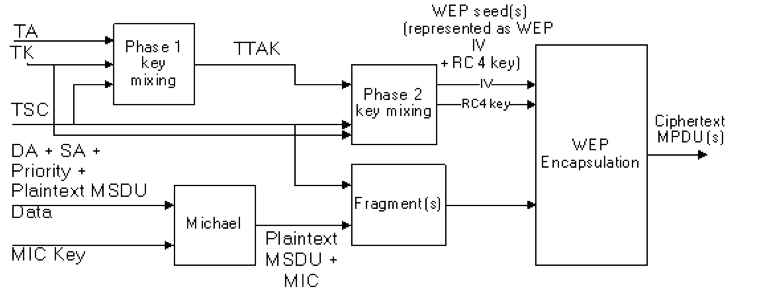
\includegraphics[width=\linewidth]{contents/background-in-wireless-networks/protected-network-standards/wpa/tkip/tkip-encapsulation-block-diagram.png}
    \caption{\gls{tkip} Encapsulation Block Diagram}
    {Source: \cite{ieee_80211_2020}}
    \label{figure:ieee80211_figure43c}
\end{figure}

Represented on Figure \ref{figure:ieee80211_figure43c}, the encryption process of \gls{tkip} combines the \gls{tk}, \gls{ta}, and \gls{tsc} using cryptographic mixing functions and uses it as the \gls{sk} and the \gls{iv} of the \gls{wep} algorithm, effectively enhancing the \gls{prng} seed strength by avoiding the reuse of keys. Then \gls{tkip} calculates the \gls{mic} by executing the Michael algorithm with the \gls{mic} key over the \gls{msdu} plaintext, priority, \gls{sa}, and \gls{da}. The result is fed to the original \gls{wep} algorithm, which outputs the \gls{mpdu} to be transmitted.

\begin{figure}[h]
    \centering
    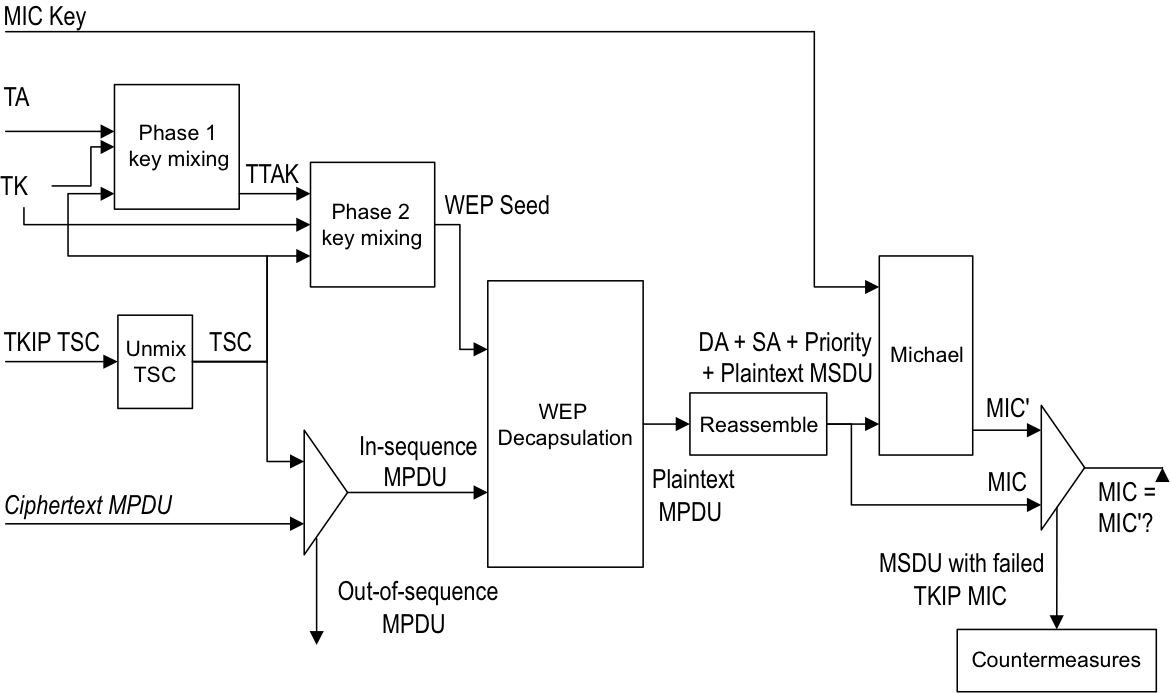
\includegraphics[width=\linewidth]{contents/background-in-wireless-networks/protected-network-standards/wpa/tkip/tkip-decapsulation-block-diagram.png}
    \caption{\gls{tkip} Decapsulation Block Diagram}
    {Source: \cite{ieee_80211_2020}}
    \label{figure:ieee80211_figure43d}
\end{figure}

When decrypting, \gls{tkip} rejects all \glspl{mpdu} received out of sequence. Then it calculates the \gls{wep} seed using the same mixing algorithm of the encryption process. The \gls{wep} algorithm is executed, decrypting the \gls{mpdu}. Michael is executed with the proper \gls{mic} key over the recently recovered data, the result is then compared to the \gls{mic} specified in the \gls{mpdu}. If the \glspl{mic} don't match, \gls{tkip} performs countermeasures procedures to mitigate what looks like an attack. Otherwise, the message is returned by the algorithm, meaning that the \gls{mpdu} was decrypted and successfully authenticated. The decryption mechanism is illustrated on Figure \ref{figure:ieee80211_figure43d}.

\FloatBarrier
